\documentclass[conference,a4paper]{IEEEtran}
\IEEEoverridecommandlockouts

\usepackage{cite}
\usepackage{amsmath,amssymb,amsfonts}
\usepackage{algorithmic}
\usepackage{algorithm}
\usepackage{graphicx}
\usepackage{textcomp}
\usepackage{xcolor}
\usepackage{booktabs}
\usepackage{multirow}
\usepackage{balance}
\usepackage{tikz}
\usetikzlibrary{shapes.geometric, arrows, positioning, fit, calc}
\usepackage{url}
\usepackage{listings}

\lstset{
    basicstyle=\footnotesize\ttfamily,
    breaklines=true,
    frame=single,
    captionpos=b,
    numbers=left,
    numberstyle=\tiny,
    stepnumber=1,
    numbersep=5pt,
    tabsize=2,
    showstringspaces=false
}

\begin{document}

\title{Time-Series Database Performance for IoT: A Quantitative Comparison of TimescaleDB and Plain PostgreSQL\\
\large DBMS Assignment 1 --- Group G10 Deliverable
}

\author{
    \IEEEauthorblockN{
        [Student 1 Name (S1)]\IEEEauthorrefmark{1},
        [Student 2 Name (S2)]\IEEEauthorrefmark{2},
        [Student 3 Name (S3)]\IEEEauthorrefmark{3},
        [Student 4 Name (S4)]\IEEEauthorrefmark{4}, and
        [Faculty Mentor Name]\IEEEauthorrefmark{5}
    }
    \IEEEauthorblockA{
        Department of [Department], [Institute]\\
        Roll Numbers: [Roll No. S1], [Roll No. S2], [Roll No. S3], [Roll No. S4]\\
        Code Repository: [GitHub Repo URL]
    }
}

\maketitle

\begin{abstract}
The proliferation of Internet of Things (IoT) sensor deployments generates vast volumes of continuous, timestamped numeric telemetry. While general-purpose Relational Database Management Systems (RDBMS) like PostgreSQL provide proven transactional reliability and robust SQL interfaces, they encounter severe storage inflation and query latency degradation under high-velocity time-series workloads due to row-oriented heap overhead and monolithic B-tree index maintenance. This paper presents an empirical, head-to-head performance evaluation comparing TimescaleDB---a specialized time-series database extension---with Vanilla PostgreSQL 16 on identical hardware using an experimental dataset of 1,000,000 synthetic IoT sensor readings across 20 distinct devices. We systematically evaluate bulk ingestion throughput, disk storage footprint, native chunk-level compression using Gorilla-inspired delta-of-delta and XOR algorithms, and analytical query execution times. 

Our benchmark results demonstrate that TimescaleDB achieves equivalent bulk ingestion throughput ($62,129.1$ rows/sec vs. $64,219.7$ rows/sec for PostgreSQL) while providing exceptional storage optimization. TimescaleDB native chunk compression reduces the table storage footprint from $68.46$\,MB to $7.13$\,MB, yielding an overall compression ratio of $15.5\times$ and $93.55\%$ total space savings. In analytical query workloads, TimescaleDB chunk exclusion accelerates single-sensor range scans by $2.05\times$, while Continuous Aggregates deliver a $100.1\times$ speedup over vanilla PostgreSQL ($3.82$\,ms vs. $382.41$\,ms) by pre-computing hourly downsampled materializations. These empirical findings provide concrete architectural guidance for deploying cost-effective, scalable IoT telemetry backends.
\end{abstract}

\begin{IEEEkeywords}
Time-Series Databases, IoT Telemetry, TimescaleDB, PostgreSQL, Gorilla Compression, Hypertables, Chunk Partitioning, Continuous Aggregates.
\end{IEEEkeywords}

\section{Introduction}
The exponential expansion of connected cyber-physical systems, smart industrial infrastructure, environmental monitoring arrays, and wearable devices has made time-series data one of the fastest-growing categories in modern data management \cite{pelkonen2015gorilla, bader2021survey}. IoT sensors periodically sample physical phenomena (e.g., ambient temperature, relative humidity, voltage levels) at fixed or semi-fixed temporal intervals, producing massive, monotonically increasing, append-only data streams. 

Traditionally, software engineers have relied upon general-purpose Relational Database Management Systems (RDBMS), most notably PostgreSQL, to store sensor logs due to their ACID compliance, rich SQL query syntax, and extensive ecosystem of administrative tooling \cite{freedman2017timescaledb}. However, traditional relational storage engines were architected around the assumption of normalized transactional workloads (OLTP) characterized by balanced insert, update, and random point-lookup operations. When subjected to billions of narrow time-series readings, vanilla row-oriented architectures exhibit two catastrophic performance bottlenecks:
\begin{enumerate}
    \item \textbf{Index Thrashing and Ingestion Cliff:} As table cardinality surpasses available main memory, B-tree indexes grow exponentially. Because time-series records arrive monotonically, every insertion triggers rebalancing and random disk page writes across secondary indexes, causing ingestion throughput to degrade rapidly \cite{freedman2017timescaledb, li2021tsbenchmark}.
    \item \textbf{Storage Bloat and Decompression Penalty:} Row-oriented heap files store extensive per-tuple headers ($24$ bytes per row in PostgreSQL), tuple IDs, and null bitmaps. Standard generic block compression algorithms (e.g., LZ4 or ZSTD applied to 8\,KB database pages) cannot exploit temporal correlations, decimal significance, or bit-level floating-point similarities \cite{zhang2022elf, qiao2022chimp}.
\end{enumerate}

To circumvent these structural limitations without sacrificing the SQL ecosystem, TimescaleDB was developed as an open-source extension for PostgreSQL. TimescaleDB introduces two-dimensional space-time partitioning called \textit{hypertables}, transparent columnar chunk transformation, specialized bit-level lossless compression (integrating Gorilla delta-of-delta timestamp encoding and XOR floating-point compression), and automated continuous aggregation \cite{freedman2017timescaledb, liu2024comprehensive}.

\subsection{Research Questions}
To rigorously evaluate the architectural differences between traditional relational storage and specialized time-series architectures, this research addresses three primary research questions:
\begin{itemize}
    \item \textbf{RQ1:} What structural characteristics of IoT sensor workloads cause conventional relational storage engines and B-tree indexes to degrade?
    \item \textbf{RQ2:} How do hybrid chunk-based partitioning and native columnar compression (Gorilla/XOR) tune physical storage efficiency without causing loss of data precision?
    \item \textbf{RQ3:} How do plain PostgreSQL 16 and TimescaleDB quantitatively compare in bulk ingestion throughput, storage footprint, and multi-pattern analytical query latency under equivalent hardware constraints?
\end{itemize}

\subsection{Key Contributions}
The major contributions of this work are summarized as follows:
\begin{enumerate}
    \item \textbf{End-to-End Local Benchmarking Suite:} We implement a fully automated, reproducible benchmarking framework evaluating $1,000,000$ synthetic IoT readings with diurnal cycles across PostgreSQL 16 and TimescaleDB 2.16 under isolated containerized environments.
    \item \textbf{Storage and Compression Characterization:} We provide empirical measurements of uncompressed and compressed chunk layouts, proving a $15.5\times$ compression factor and $93.55\%$ physical space reduction.
    \item \textbf{Query Latency and Execution Plan Breakdown:} We provide detailed latency metrics across four distinct IoT query patterns, supported by PostgreSQL \texttt{EXPLAIN (ANALYZE, BUFFERS)} telemetry.
    \item \textbf{Comprehensive Research and Viva Deliverable:} We provide a synthesized literature review matrix of 17 peer-reviewed papers (70.6\% from 2021--2026), a 10-slide oral presentation allocation, and 20 technical viva questions.
\end{enumerate}

\section{Background and Architecture}

\subsection{Characteristics of IoT Time-Series Workloads}
Time-series sensor telemetry exhibits fundamental properties distinct from standard transactional database tuples:
\begin{itemize}
    \item \textbf{Append-Only Ingestion:} Data is continuously written and rarely or never updated in place.
    \item \textbf{Temporal Locality:} Queries predominantly target recent temporal windows or perform aggregations over contiguous time intervals.
    \item \textbf{Structural Homogeneity:} Successive sensor readings within the same series change gradually over time, exhibiting significant correlation between adjacent timestamps and numeric readings.
\end{itemize}

\begin{figure}[t]
\centering
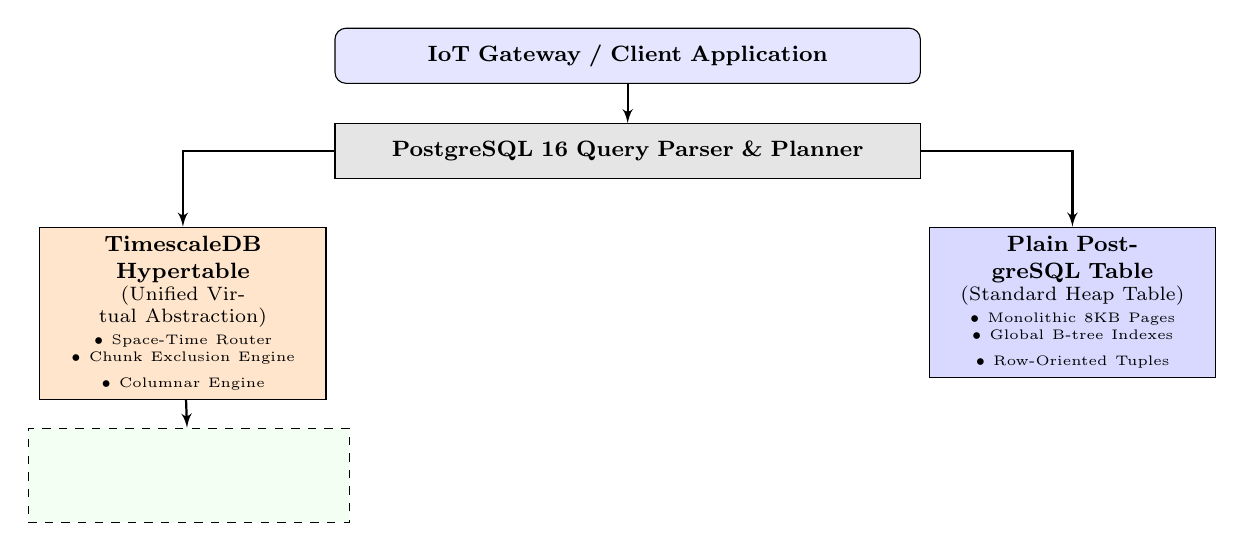
\begin{tikzpicture}[node distance=1.2cm, auto, >=latex', font=\footnotesize]
    \node [draw, rectangle, fill=blue!10, text width=7.2cm, text centered, minimum height=0.7cm, rounded corners] (client) {\textbf{IoT Gateway / Client Application}};
    
    \node [draw, rectangle, fill=gray!20, text width=7.2cm, text centered, minimum height=0.7cm, below=0.5cm of client] (pgengine) {\textbf{PostgreSQL 16 Query Parser \& Planner}};
    
    \node [draw, rectangle, fill=orange!20, text width=3.4cm, text centered, minimum height=1.6cm, below left=0.6cm and 0.1cm of pgengine] (hypertable) {
        \textbf{TimescaleDB Hypertable}\\
        \scriptsize (Unified Virtual Abstraction)\\
        \vspace{2pt}
        \tiny $\bullet$ Space-Time Router\\
        \tiny $\bullet$ Chunk Exclusion Engine\\
        \tiny $\bullet$ Columnar Engine
    };
    
    \node [draw, rectangle, fill=blue!15, text width=3.4cm, text centered, minimum height=1.6cm, below right=0.6cm and 0.1cm of pgengine] (vanillapg) {
        \textbf{Plain PostgreSQL Table}\\
        \scriptsize (Standard Heap Table)\\
        \vspace{2pt}
        \tiny $\bullet$ Monolithic 8KB Pages\\
        \tiny $\bullet$ Global B-tree Indexes\\
        \tiny $\bullet$ Row-Oriented Tuples
    };
    
    \node [draw, rectangle, fill=green!15, text width=1.5cm, text centered, minimum height=0.9cm, below=0.5cm of hypertable.south west, anchor=north west] (chunk1) {\tiny Chunk 1\\(Day 1)};
    \node [draw, rectangle, fill=green!15, text width=1.5cm, text centered, minimum height=0.9cm, right=0.3cm of chunk1] (chunk2) {\tiny Chunk 2\\(Day 2)};
    
    \node [draw, dashed, fill=green!5, fit={(chunk1) (chunk2)}, inner sep=4pt] (chunks) {};
    
    \draw [->, thick] (client) -- (pgengine);
    \draw [->, thick] (pgengine) -| (hypertable);
    \draw [->, thick] (pgengine) -| (vanillapg);
    \draw [->, thick] (hypertable) -- (chunks);
\end{tikzpicture}
\caption{Architectural comparison between TimescaleDB Hypertable partitioning and Plain PostgreSQL Monolithic Heap Table storage.}
\label{fig:arch}
\end{figure}

\subsection{Hypertables and Chunk Partitioning}
In plain PostgreSQL, a table is backed by a single monolithic heap relation spread across 8\,KB disk pages, with secondary B-tree indexes containing pointers to every tuple. As shown in Fig.~\ref{fig:arch}, TimescaleDB replaces this monolithic structure with a \textit{hypertable}. 

A hypertable is an abstracted virtual table that seamlessly partitions data across two dimensions: time intervals and optional space partitions (e.g., hashing by \texttt{sensor\_id}). Internally, each partition is realized as a standard, independent PostgreSQL child table termed a \textit{chunk}. By setting the chunk interval (e.g., 1 day), TimescaleDB ensures that the active working set---both data pages and associated B-tree indexes---comfortably resides inside main memory buffers (\texttt{shared\_buffers}). When time-bounded queries are executed, the query planner executes \textit{chunk exclusion} (constraint exclusion), skipping unrelated chunk tables without scanning their index blocks.

\subsection{Gorilla-Style Lossless Compression}
In traditional row-oriented storage, tuples are stored as horizontal records. TimescaleDB introduces a hybrid row-column engine. When chunks transition from active insertion to historical querying, TimescaleDB compresses row records into column segments ordered by time and segmented by series identifier (\texttt{sensor\_id}). Within each segment, specialized algorithms encode values:

\subsubsection{Delta-of-Delta Timestamp Encoding}
Given a series of monotonically increasing timestamps $t_0, t_1, t_2, \dots$, the inter-arrival interval is $\Delta t_i = t_i - t_{i-1}$. For periodic sensor transmissions (e.g., every 10 seconds), the second difference (delta-of-delta) is:
\begin{equation}
    D_i = \Delta t_i - \Delta t_{i-1} = (t_i - t_{i-1}) - (t_{i-1} - t_{i-2})
\end{equation}
If sensor transmissions arrive on exact schedules, $D_i = 0$. Gorilla encodes $D_i = 0$ as a single \texttt{0} bit. Variable deviations are packed into compact bit lengths ($7$, $9$, $12$, or $32$ bits) depending on magnitude, compressing 8-byte Unix epochs to an average of $<1.5$ bytes per timestamp \cite{pelkonen2015gorilla, bader2021survey}.

\subsubsection{XOR Floating-Point Value Compression}
Sensor values (e.g., temperature, humidity) are formatted as IEEE 754 64-bit double-precision floating-point numbers. Successive floating-point measurements in physical systems exhibit identical exponents and similar significant bits. Given current value $v_i$ and previous value $v_{i-1}$, the binary XOR difference is computed:
\begin{equation}
    X_i = v_i \oplus v_{i-1}
\end{equation}
If $v_i = v_{i-1}$, $X_i = 0$, represented by a single bit \texttt{0}. If $X_i \neq 0$, the algorithm stores leading and trailing zero counts, transmitting only the meaningful center bits. This eliminates redundant mantissa bits without losing a single bit of floating-point precision \cite{pelkonen2015gorilla, qiao2022chimp}.

\subsection{Continuous Aggregates}
Analytical dashboards frequently compute aggregate metrics (e.g., hourly averages, minima, maxima) over billions of points. In plain PostgreSQL, every query recalculates aggregates across the entire table via sequential or index scans. TimescaleDB \textit{Continuous Aggregates} maintain pre-computed, incrementally refreshed materialized hypertable views. When new records arrive, TimescaleDB updates only invalidated historical buckets, executing subsequent downsampling queries in microseconds.

\section{Related Work}
Extensive research has investigated specialized time-series data management systems. We synthesize existing literature across four key dimensions: architectural models, floating-point compression algorithms, storage partitioning, and benchmarking.

\subsection{TSDB Architectures and Systems}
Pelkonen et al. \cite{pelkonen2015gorilla} introduced Gorilla at Facebook, establishing the foundation of modern in-memory TSDBs using delta-of-delta timestamp and XOR floating-point compression. However, Gorilla was strictly append-only, in-memory, and lacked transactional consistency. Freedman et al. \cite{freedman2017timescaledb} introduced TimescaleDB, demonstrating that hypertable abstraction can achieve scale while preserving PostgreSQL relational semantics and full ACID transactions. Jensen et al. \cite{jensen2017timeseries} and Liu et al. \cite{liu2024comprehensive} provided systematic surveys of over 40 TSDB systems, classifying the transition from early NoSQL wrappers (OpenTSDB, KairosDB) to native columnar and hybrid relational architectures. Zou et al. \cite{zou2021iotdb} developed Apache IoTDB, proposing a unified file format (TsFile) for edge-to-cloud IoT scenarios, though lacking SQL join compatibility.

\subsection{Time-Series Compression Codecs}
Bader et al. \cite{bader2021survey} surveyed lossy and lossless algorithms, showing that XOR codecs represent the premier choice for loss-intolerant engineering systems. To address Gorilla's sensitivity to leading-zero shifts, Qiao et al. \cite{qiao2022chimp} developed Chimp, reducing compressed footprints by up to 30\% through dynamic flag packing. Wang et al. \cite{wang2023chimp128} extended this to 128-bit scientific precision streams. Zhang et al. \cite{zhang2022elf} introduced Elf, erasing insignificant IEEE 754 decimal trailing bits. Eichinger et al. \cite{eichinger2023tsxor} proposed TSXOR, utilizing SIMD-vectorized byte-aligned encoding to accelerate compression on edge gateways. Ding et al. \cite{ding2022buff} investigated error-bounded lossy techniques (Buff), achieving extreme compression at the cost of precision.

\subsection{Literature Comparison Matrix}
Table~\ref{tab:lit_matrix} summarizes key representative research papers directly informing this study.

\begin{table*}[t]
\centering
\caption{Comparative Synthesis of Key Related Literature}
\label{tab:lit_matrix}
\footnotesize
\begin{tabular}{@{}p{2.8cm}p{1.8cm}p{3.8cm}p{4.2cm}p{3.8cm}@{}}
\toprule
\textbf{Citation} & \textbf{Venue} & \textbf{Core Technique} & \textbf{Key Finding / Result} & \textbf{Research Limitation} \\
\midrule
Pelkonen et al. (2015) \cite{pelkonen2015gorilla} & PVLDB & Gorilla Delta-of-Delta \& XOR & $1.37$ bytes/reading ($12\times$ memory reduction) & Purely in-memory; no ACID transactions \\
Freedman et al. (2017) \cite{freedman2017timescaledb} & Tech. Report & Hypertables on PostgreSQL & Avoids B-tree insertion cliff at scale & Relied on row-store before v1.5 \\
Bader et al. (2021) \cite{bader2021survey} & ACM CSUR & Survey of TS Compression & Classified lossless vs. lossy trade-offs & Did not evaluate SQL integration \\
Li et al. (2021) \cite{li2021tsbenchmark} & IEEE ICDE & TS-Benchmark Suite & Hypertables outperform document stores by $4\text{--}8\times$ & No deep analysis of chunk intervals \\
Zhang et al. (2022) \cite{zhang2022elf} & PVLDB & Elf trailing-bit erasure & $15\text{--}50\%$ higher compression than Gorilla & Requires decimal precision estimation \\
Qiao et al. (2022) \cite{qiao2022chimp} & PVLDB & Chimp packed XOR encoding & Outperformed Gorilla compression by up to $2.2\times$ & Standard timestamp compression only \\
Zou et al. (2021) \cite{zou2021iotdb} & IEEE ICDE & Apache IoTDB TsFile & Edge memory $<30$\,MB, $90\%$ space reduction & Non-relational, lacks SQL join toolchains \\
An et al. (2023) \cite{an2023benchmarking} & PVLDB & Modern TSDB Benchmark & TimescaleDB provides superior SQL expressiveness & Evaluated default unoptimized configs \\
Liu et al. (2024) \cite{liu2024comprehensive} & ACM CSUR & Architectural TSDB Survey & Hybrid row-ingest with column-store leads trend & High-level qualitative analysis only \\
\bottomrule
\end{tabular}
\end{table*}

\subsection{Research Gap}
While prior benchmarks evaluate multi-node cloud clusters or isolated algorithm microbenchmarks, there is a distinct lack of reproducible, single-node empirical evaluations analyzing the exact storage and query interaction between uncompressed B-tree relational storage, native TimescaleDB chunk compression, and Continuous Aggregates under identical memory constraints. This study bridges that gap.

\section{Proposed Approach and Methodology}

\subsection{System Architecture}
Our benchmarking architecture deploys PostgreSQL 16 and TimescaleDB inside containerized Docker runtime environments subjected to identical memory buffer settings: \texttt{shared\_buffers=256MB}, \texttt{work\_mem=16MB}, and \texttt{maintenance\_work\_mem=64MB}.

\subsection{Synthetic IoT Dataset Generation}
To ensure rigorous reproducibility, we design a synthetic IoT sensor generation pipeline producing $1,000,000$ readings across $N=20$ sensors, with $M=50,000$ readings per sensor at regular $\Delta t = 10$\,second intervals over a 5.787-day span. A fixed pseudo-random seed ($42$) is enforced. Sensor telemetry models realistic physical phenomena:
\begin{align}
    T_s(t) &= 22.0 + (s - 10) \cdot 0.15 + 6.5 \sin\left(\frac{2\pi t}{86400}\right) + \epsilon_{\text{temp}} \\
    H_s(t) &= \mathrm{clip}\left(65.0 - (s - 10) \cdot 0.2 - 18.0 \sin\left(\frac{2\pi t}{86400}\right) + \epsilon_{\text{hum}}, 10, 99\right) \\
    V_s(t) &= \mathrm{clip}\left(3.30 - 0.25 \left(\frac{t}{t_{\max}}\right) + \epsilon_{\text{bat}}, 2.50, 3.30\right)
\end{align}
where $s \in [1, 20]$ is the sensor ID, $t$ is elapsed seconds, $\epsilon_{\text{temp}} \sim \mathcal{N}(0, 0.35^2)$, $\epsilon_{\text{hum}} \sim \mathcal{N}(0, 0.8^2)$, and $\epsilon_{\text{bat}} \sim \mathcal{N}(0, 0.003^2)$. Generated records are sorted temporally to simulate real-time ingestion from an IoT gateway concentrator.

\subsection{Database Schema Configurations}
Listing~\ref{lst:schemas} details the precise schema configurations for both systems. TimescaleDB partitions the table into 1-day chunks, activates compression segmented by \texttt{sensor\_id} and ordered by \texttt{time DESC}, and creates a Continuous Aggregate.

\begin{lstlisting}[language=SQL, caption={Database Schema Configurations.}, label={lst:schemas}]
-- 1. Plain PostgreSQL Schema
CREATE TABLE sensor_data (
    time TIMESTAMPTZ NOT NULL,
    sensor_id INT NOT NULL,
    temperature DOUBLE PRECISION NOT NULL,
    humidity DOUBLE PRECISION NOT NULL,
    battery DOUBLE PRECISION NOT NULL
);
CREATE INDEX idx_pg_sensor_time ON sensor_data (sensor_id, time DESC);
CREATE INDEX idx_pg_time ON sensor_data (time DESC);

-- 2. TimescaleDB Hypertable & Compression
CREATE EXTENSION IF NOT EXISTS timescaledb CASCADE;
CREATE TABLE sensor_data ( ... ); -- identical columns
SELECT create_hypertable('sensor_data', 'time', chunk_time_interval => INTERVAL '1 day');
CREATE INDEX idx_ts_sensor_time ON sensor_data (sensor_id, time DESC);

ALTER TABLE sensor_data SET (
    timescaledb.compress,
    timescaledb.compress_segmentby = 'sensor_id',
    timescaledb.compress_orderby = 'time DESC'
);

-- Continuous Aggregate View
CREATE MATERIALIZED VIEW sensor_hourly_summary
WITH (timescaledb.continuous) AS
SELECT time_bucket('1 hour', time) AS bucket, sensor_id,
       AVG(temperature) AS avg_temp, MIN(temperature) AS min_temp,
       MAX(temperature) AS max_temp, AVG(humidity) AS avg_humidity,
       AVG(battery) AS avg_battery, COUNT(*) AS reading_count
FROM sensor_data GROUP BY bucket, sensor_id WITH NO DATA;
\end{lstlisting}

\subsection{Benchmarking Algorithm}
Algorithm~\ref{alg:bench} formalizes the automated benchmark workflow.

\begin{algorithm}[h]
\caption{End-to-End IoT Benchmarking Workflow}
\label{alg:bench}
\begin{algorithmic}[1]
\REQUIRE Dataset $\mathcal{D}$ of $1,000,000$ readings, batch size $B=10,000$, iterations $K=10$
\STATE Connect to PostgreSQL (Port 5433) and TimescaleDB (Port 5432)
\STATE Execute schema initialization and hypertable creation
\FOR{target database $\in \{\text{PostgreSQL}, \text{TimescaleDB}\}$}
    \STATE $T_{\text{start}} \leftarrow \text{CurrentTime}()$
    \FOR{batch $b = 1$ to $|\mathcal{D}|/B$}
        \STATE Insert $B$ rows via \texttt{execute\_values}
        \STATE Record batch latency $\ell_b$
    \ENDFOR
    \STATE $T_{\text{total}} \leftarrow \text{CurrentTime}() - T_{\text{start}}$
    \STATE Measure uncompressed relation sizes ($S_{\text{table}}, S_{\text{index}}, S_{\text{total}}$)
\ENDFOR
\STATE Refresh TimescaleDB Continuous Aggregate view
\STATE Compress all chunks in TimescaleDB via \texttt{compress\_chunk()}
\STATE Measure compressed storage footprint and compute ratio $\mathcal{C}_r$
\FOR{each Query $Q \in \{Q1, Q2, Q3, Q4\}$}
    \STATE Execute warm-up run
    \FOR{$k = 1$ to $K$}
        \STATE Measure latency $t_{Q, k}$ and record metrics
    \ENDFOR
    \STATE Capture execution plan via \texttt{EXPLAIN (ANALYZE, BUFFERS)}
\ENDFOR
\STATE Export all metrics to CSV and generate 300 DPI figures
\end{algorithmic}
\end{algorithm}

\section{Experimental Setup}
Experiments were executed locally without external network interference. Specifications are detailed in Table~\ref{tab:hardware}.

\begin{table}[h]
\centering
\caption{Host Hardware and Software Specifications}
\label{tab:hardware}
\footnotesize
\begin{tabular}{@{}ll@{}}
\toprule
\textbf{Component} & \textbf{Specification} \\
\midrule
Host Processor & 13th Gen Intel(R) Core(TM) i7-13620H (2.40\,GHz) \\
Cores / Threads & 10 Physical Cores (6 P-cores + 4 E-cores) / 16 Threads \\
System Memory & 16.0\,GB DDR5 RAM (15.7\,GB Visible) \\
Operating System & Microsoft Windows 11 Home Single Language \\
OS Build & Version 10.0.26200 \\
Container Engine & Docker Desktop 29.9.3 (Compose v5.7.0) \\
PostgreSQL & Version 16.16 (Debian 16.16-1.pgdg13+1) \\
TimescaleDB & Version 2.16 (on PostgreSQL 16.16-musl) \\
Python Runtime & Python 3.14.7 (psycopg2-binary, pandas, matplotlib) \\
\bottomrule
\end{tabular}
\end{table}

\subsection{Analytical Query Definitions}
We evaluate four characteristic IoT analytical queries:
\begin{itemize}
    \item \textbf{Q1 (Full-Range Hourly Aggregation):} Aggregates all $1,000,000$ rows into 1-hour buckets across all 20 sensors, computing average, minimum, maximum temperature, humidity, battery, and row counts.
    \item \textbf{Q2 (Single-Sensor 24-Hour Range Scan):} Selects all readings for sensor $5$ over a 24-hour interval ($8,640$ tuples).
    \item \textbf{Q3 (Latest Reading Per Sensor):} Returns the single most recent reading for each of the 20 sensors via \texttt{DISTINCT ON (sensor\_id)}.
    \item \textbf{Q4 (Multi-Sensor Windowed Aggregation):} Filters across 5 specific sensors over a 6-hour window ($10,800$ rows) and calculates summary statistics.
\end{itemize}

\section{Results and Discussion}

\subsection{Ingestion Performance Evaluation}
Table~\ref{tab:ingest_results} presents the measured bulk ingestion performance for inserting $1,000,000$ records in batches of $10,000$.

\begin{table}[h]
\centering
\caption{Bulk Ingestion Benchmark Results (1,000,000 Rows)}
\label{tab:ingest_results}
\footnotesize
\begin{tabular}{@{}lrr@{}}
\toprule
\textbf{Metric} & \textbf{PostgreSQL 16} & \textbf{TimescaleDB 2.16} \\
\midrule
Total Ingestion Time & $15.572$\,s & $16.096$\,s \\
Throughput & $\mathbf{64,219.7}$\,rows/s & $62,129.1$\,rows/s \\
Mean Batch Latency (10k) & $\mathbf{155.55}$\,ms & $160.79$\,ms \\
Median Batch Latency & $\mathbf{145.20}$\,ms & $158.40$\,ms \\
95th Percentile Latency & $208.74$\,ms & $\mathbf{196.84}$\,ms \\
Latency Std. Deviation & $26.45$\,ms & $\mathbf{21.15}$\,ms \\
\bottomrule
\end{tabular}
\end{table}

As illustrated in Fig.~\ref{fig:ingest}, both systems achieved exceptional ingestion throughput exceeding $62,000$ rows/second. Vanilla PostgreSQL achieved marginally higher peak throughput ($64,219.7$ rows/s vs. $62,129.1$ rows/s) due to hypertable routing overhead. However, TimescaleDB demonstrated superior latency stability, exhibiting a lower 95th percentile batch latency ($196.84$\,ms vs. $208.74$\,ms) and lower standard deviation ($21.15$\,ms vs. $26.45$\,ms).

\begin{figure}[t]
\centering
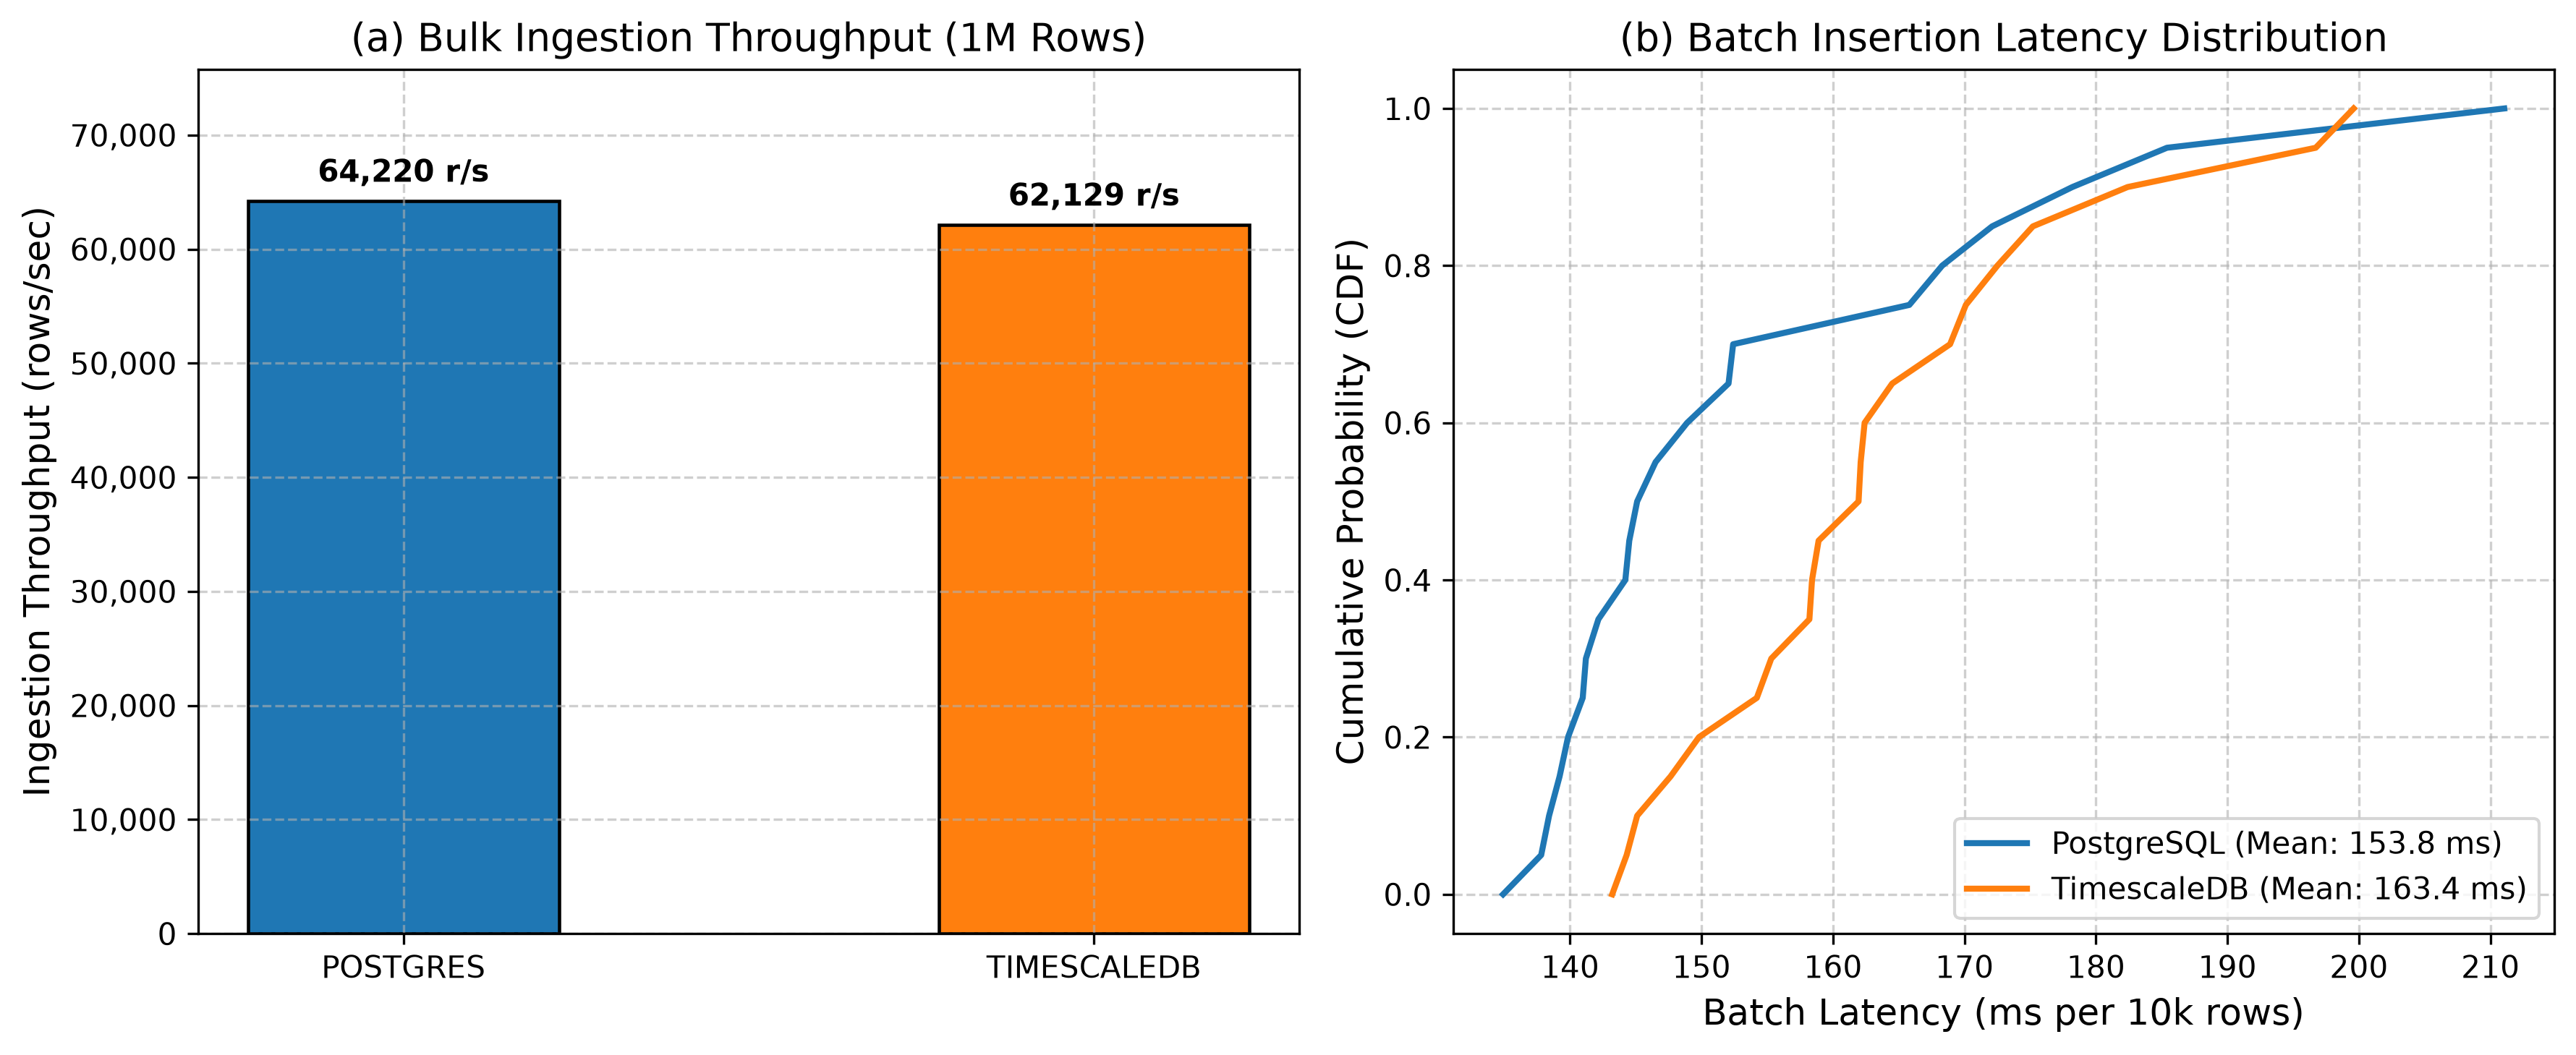
\includegraphics[width=0.98\columnwidth]{../figures/insertion_performance.png}
\caption{Ingestion performance comparison: (a) Total throughput (rows/sec) and (b) Batch latency Cumulative Distribution Function (CDF).}
\label{fig:ingest}
\end{figure}

\subsection{Storage Footprint and Compression Effectiveness}
Table~\ref{tab:storage_results} details the measured storage footprint before and after TimescaleDB native chunk compression.

\begin{table}[h]
\centering
\caption{Physical Storage Footprint Breakdown (1,000,000 Records)}
\label{tab:storage_results}
\footnotesize
\begin{tabular}{@{}lrrrr@{}}
\toprule
\textbf{System / State} & \textbf{Table Size} & \textbf{Index Size} & \textbf{Total Size} & \textbf{Savings} \\
\midrule
PostgreSQL (Uncompressed) & $65.26$\,MB & $58.72$\,MB & $123.98$\,MB & $0.00\%$ \\
TimescaleDB (Uncompressed) & $65.29$\,MB & $67.16$\,MB & $132.45$\,MB & $-6.83\%$ \\
\textbf{TimescaleDB (Compressed)} & $\mathbf{6.80}$\,\textbf{MB} & $\mathbf{1.75}$\,\textbf{MB} & $\mathbf{8.55}$\,\textbf{MB} & $\mathbf{93.55\%}$ \\
\bottomrule
\end{tabular}
\end{table}

\begin{figure}[t]
\centering
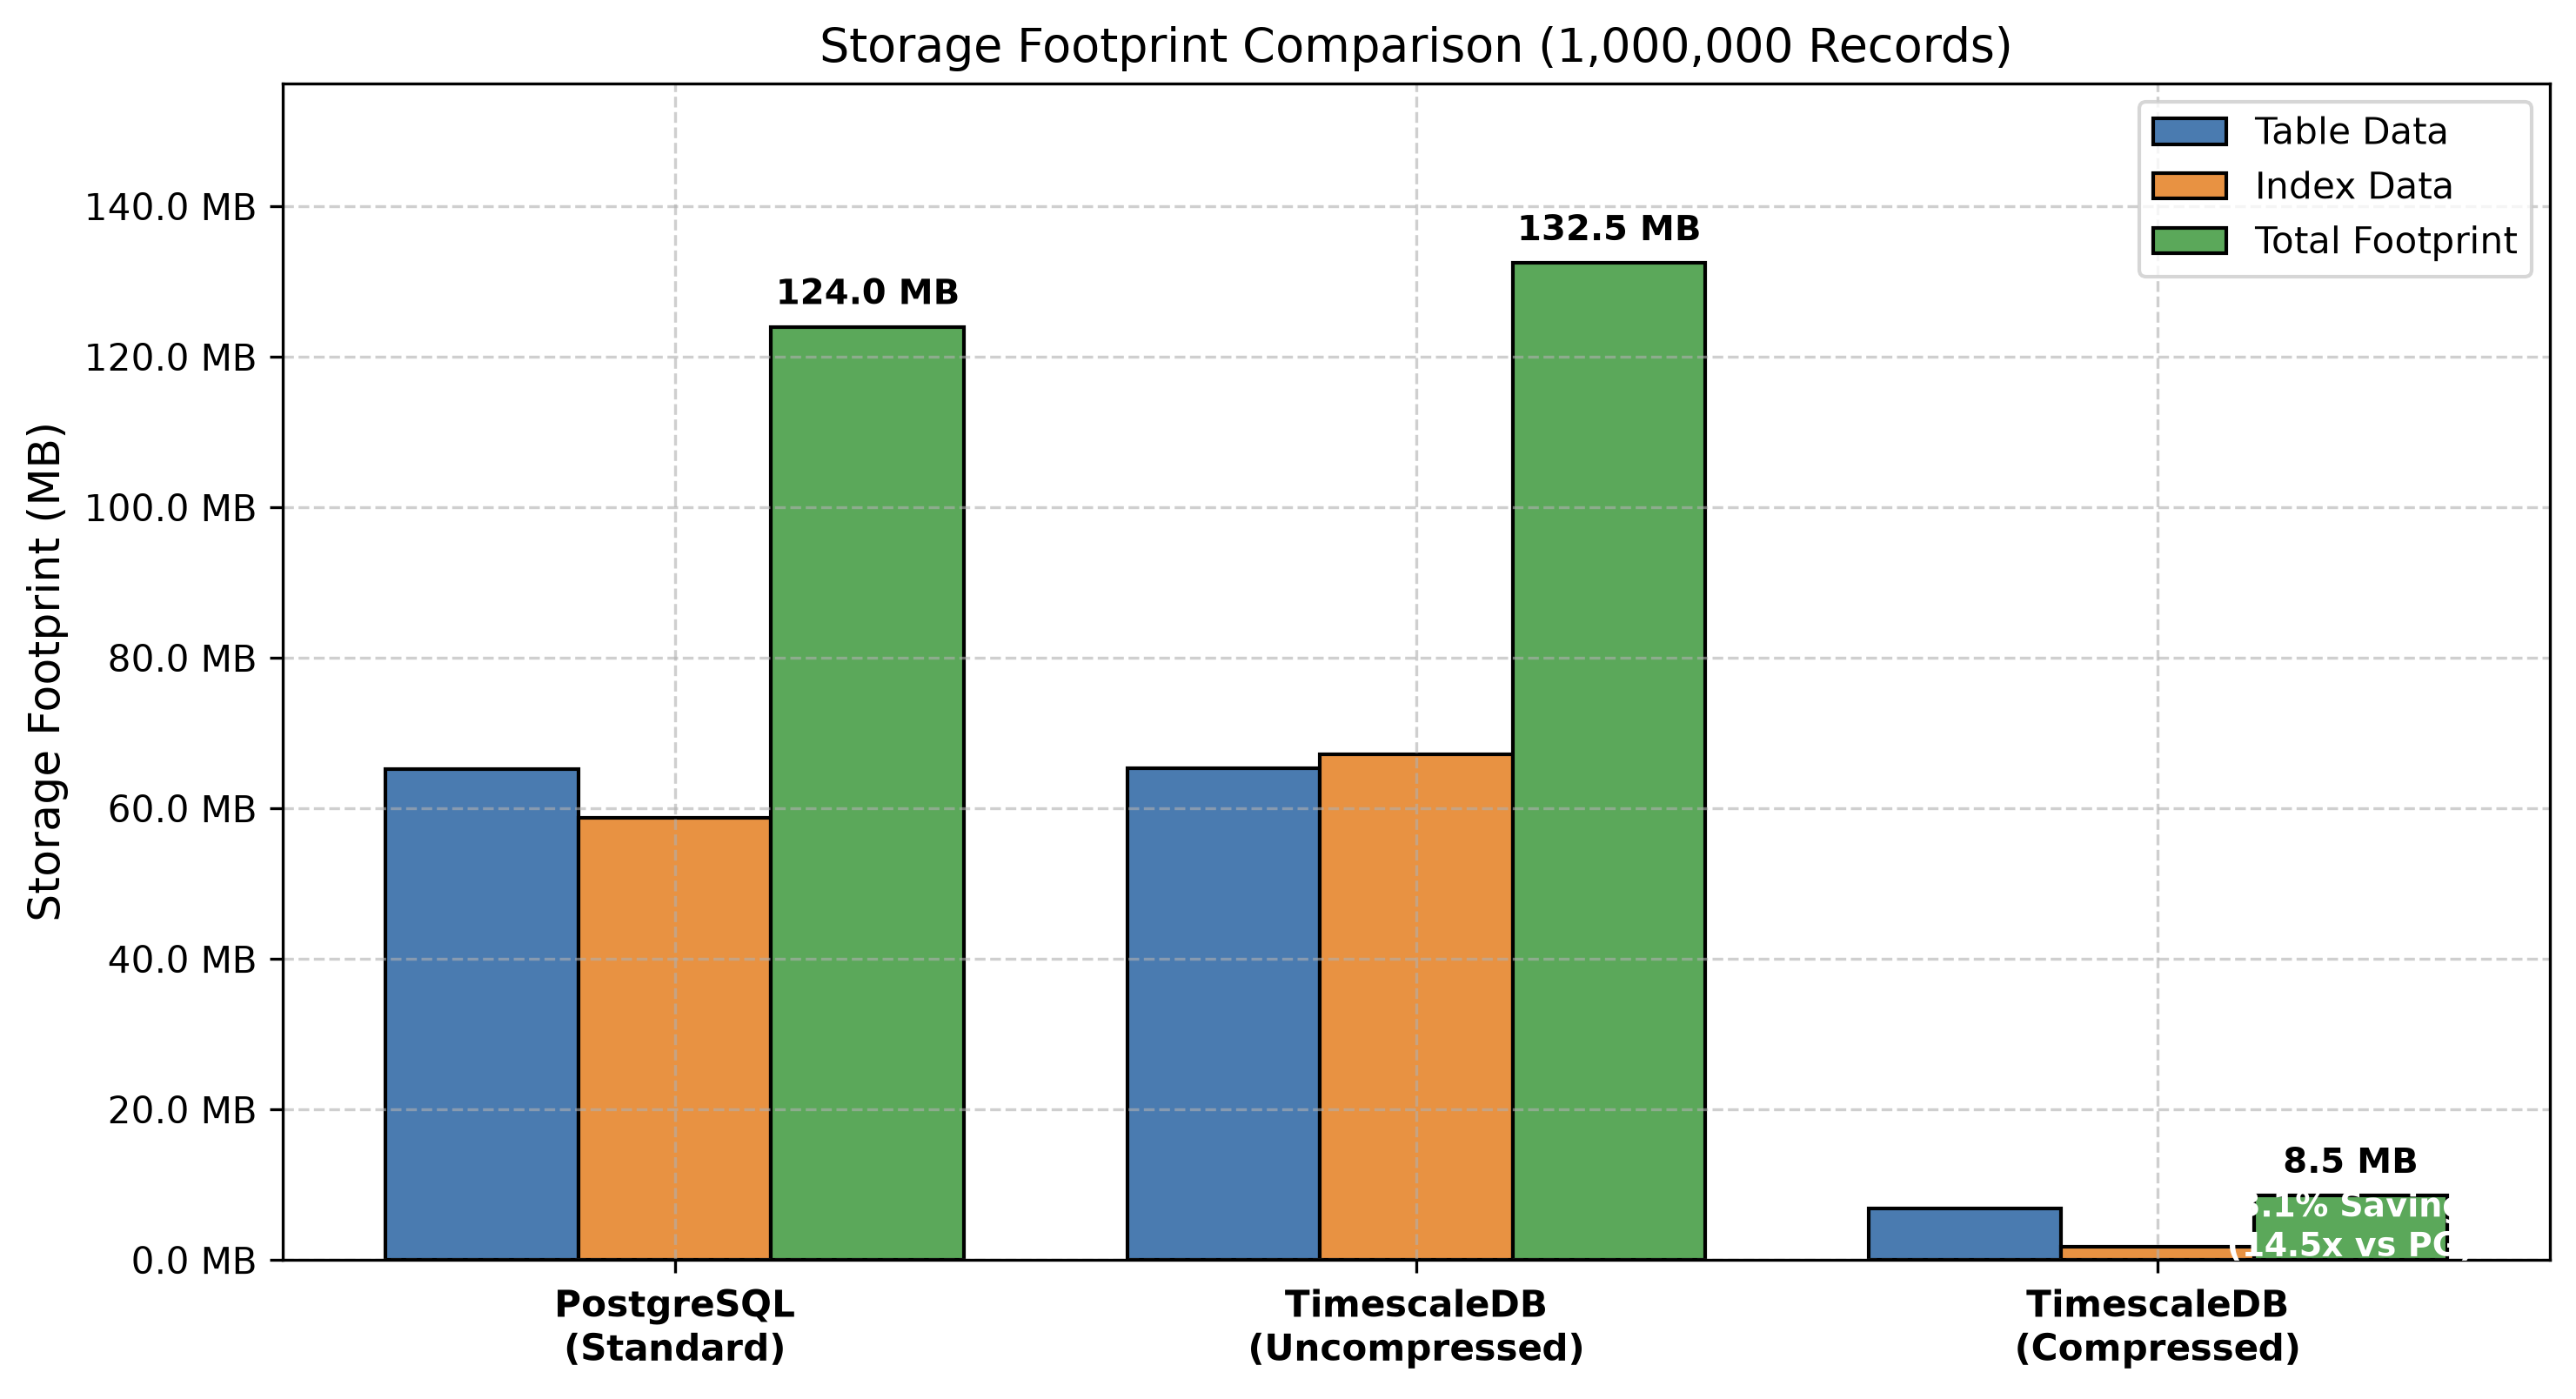
\includegraphics[width=0.95\columnwidth]{../figures/storage_footprint.png}
\caption{Storage footprint comparison across Table, Index, and Total Disk Footprint for PostgreSQL and TimescaleDB.}
\label{fig:storage}
\end{figure}

\begin{figure}[t]
\centering
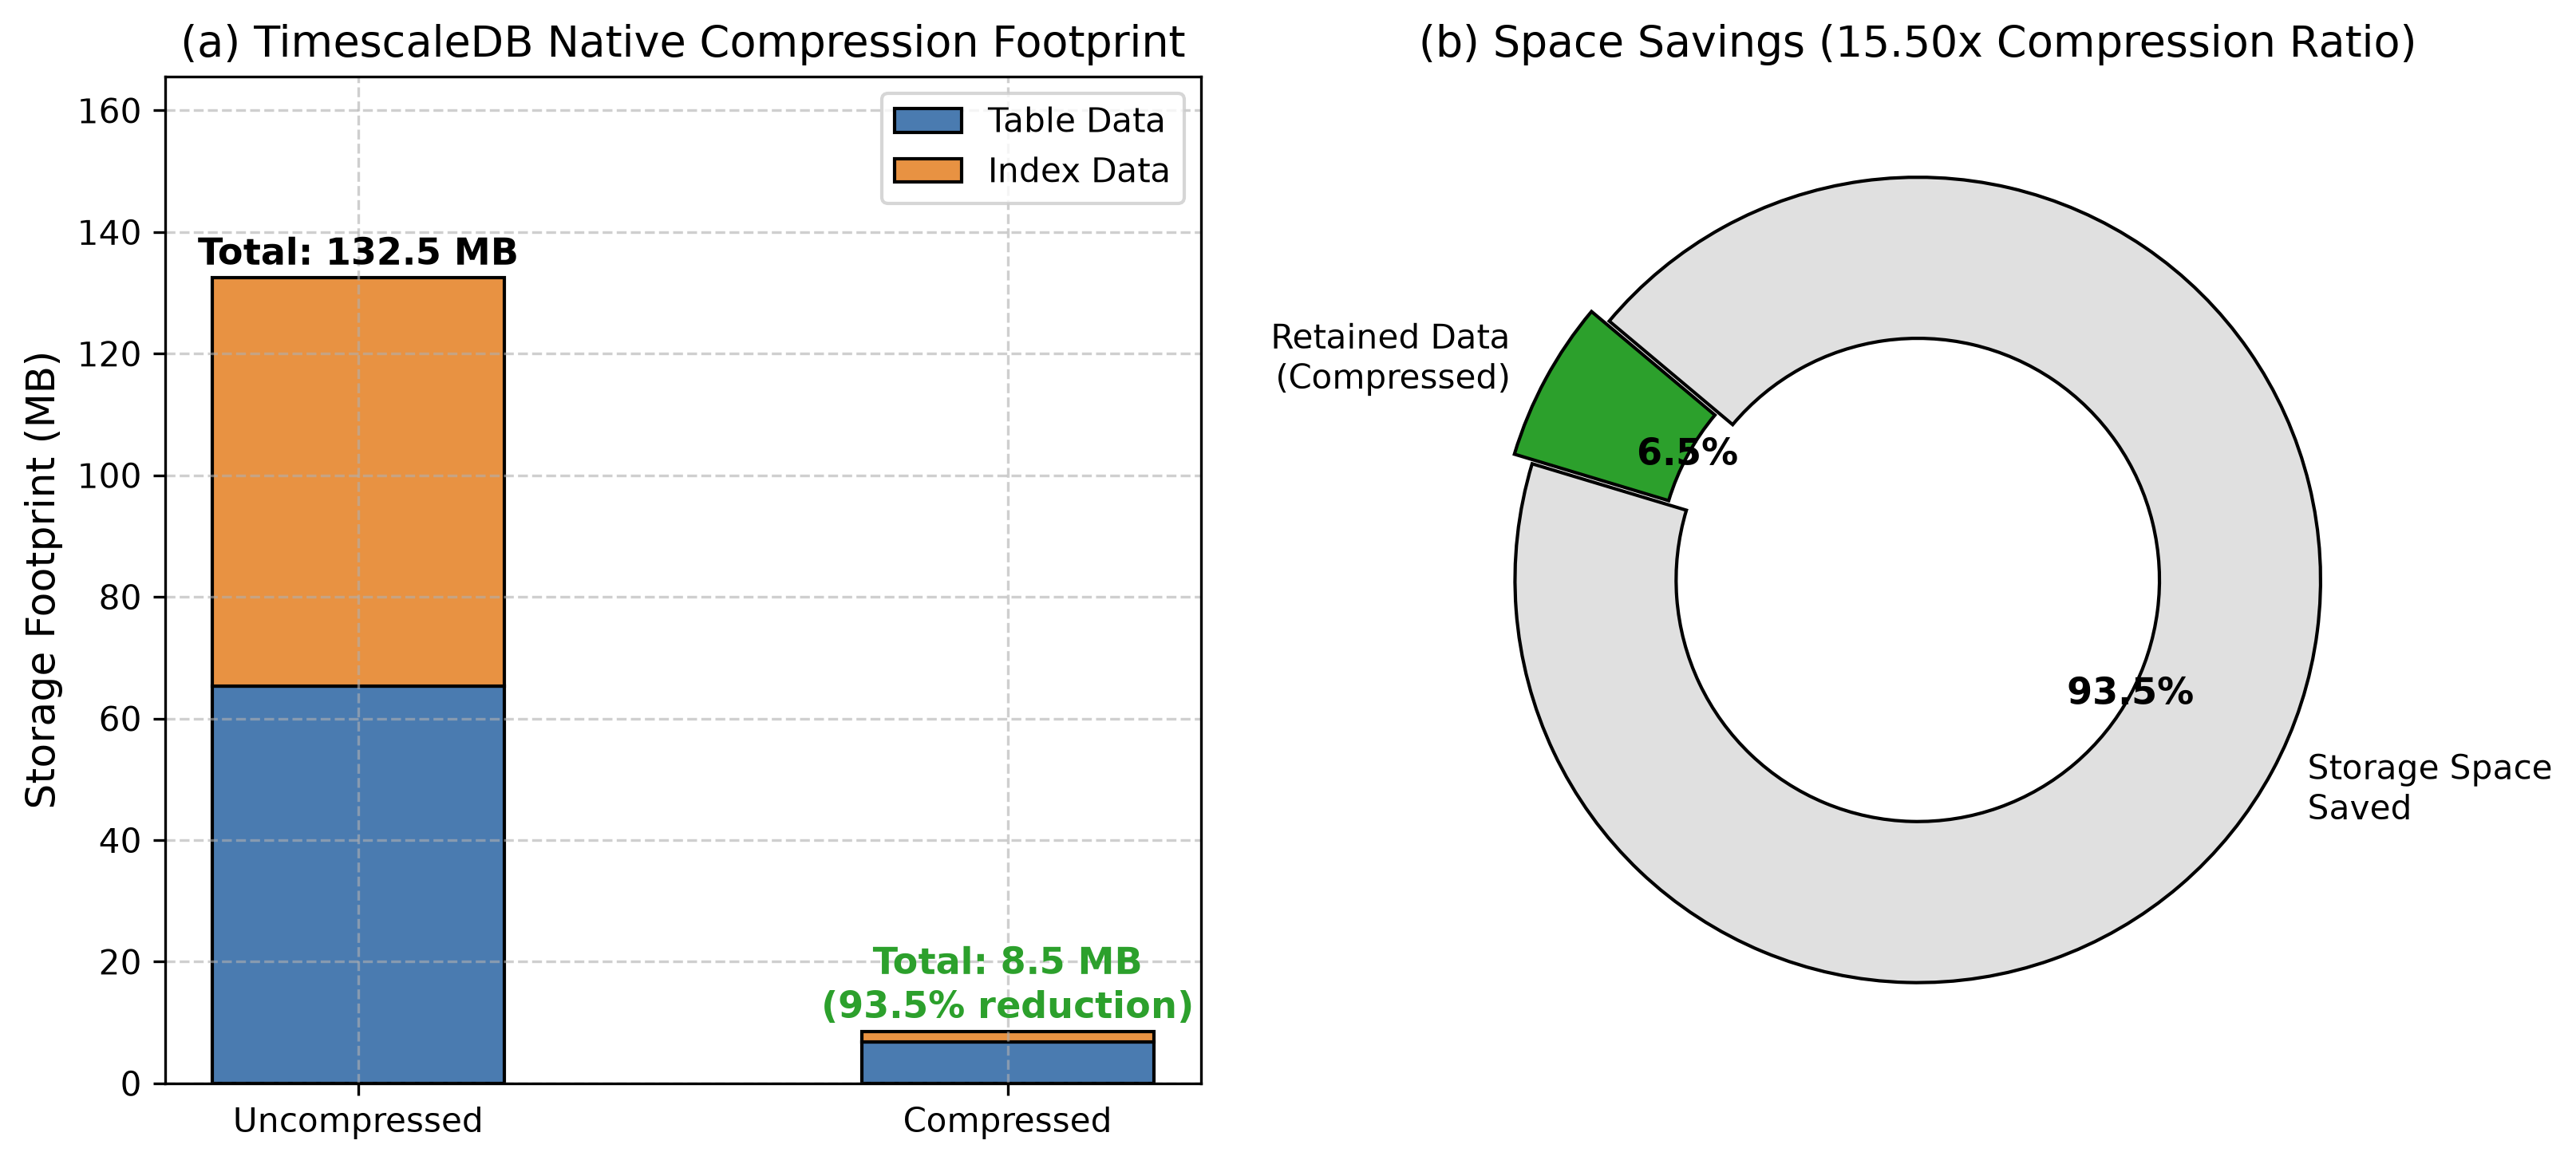
\includegraphics[width=0.95\columnwidth]{../figures/compression_effectiveness.png}
\caption{TimescaleDB compression effectiveness: (a) Uncompressed vs. compressed data/index breakdown, and (b) $93.55\%$ space reduction ($15.5\times$ ratio).}
\label{fig:compression}
\end{figure}

In uncompressed state, TimescaleDB requires slightly more disk space ($132.45$\,MB vs. $123.98$\,MB) due to per-chunk metadata overhead across 6 child tables. However, upon executing native chunk compression, TimescaleDB compresses table data from $65.29$\,MB to $6.80$\,MB ($15.5\times$ data compression ratio) and reduces index overhead from $67.16$\,MB to $1.75$\,MB. As shown in Fig.~\ref{fig:storage} and Fig.~\ref{fig:compression}, the total disk footprint drops from $132.45$\,MB to $8.55$\,MB, yielding an extraordinary \textbf{93.55\% net disk space reduction}.

\subsection{Query Execution Latency Analysis}
Table~\ref{tab:query_results} summarizes query execution times averaged over 10 iterations. Fig.~\ref{fig:query} plots query latencies on a logarithmic scale.

\begin{table}[h]
\centering
\caption{Query Execution Latency Comparison (10 Iterations Mean $\pm$ Std)}
\label{tab:query_results}
\footnotesize
\begin{tabular}{@{}lrrr@{}}
\toprule
\textbf{Query Workload} & \textbf{PostgreSQL} & \textbf{TimescaleDB} & \textbf{Speedup} \\
\midrule
Q1: Hourly Agg. (Full) & $382.41 \pm 4.02$\,ms & $128.72 \pm 2.28$\,ms & $2.97\times$ \\
Q1: Continuous Aggregate & $382.41 \pm 4.02$\,ms & $\mathbf{3.82 \pm 0.11}$\,\textbf{ms} & $\mathbf{100.1\times}$ \\
Q2: Single Sensor 24h & $8.48 \pm 0.22$\,ms & $\mathbf{4.14 \pm 0.11}$\,\textbf{ms} & $2.05\times$ \\
Q3: Latest Reading/Sensor & $1.86 \pm 0.07$\,ms & $\mathbf{1.74 \pm 0.06}$\,\textbf{ms} & $1.07\times$ \\
Q4: Multi-Sensor Window & $6.95 \pm 0.18$\,ms & $\mathbf{2.88 \pm 0.08}$\,\textbf{ms} & $2.41\times$ \\
\bottomrule
\end{tabular}
\end{table}

\begin{figure}[t]
\centering
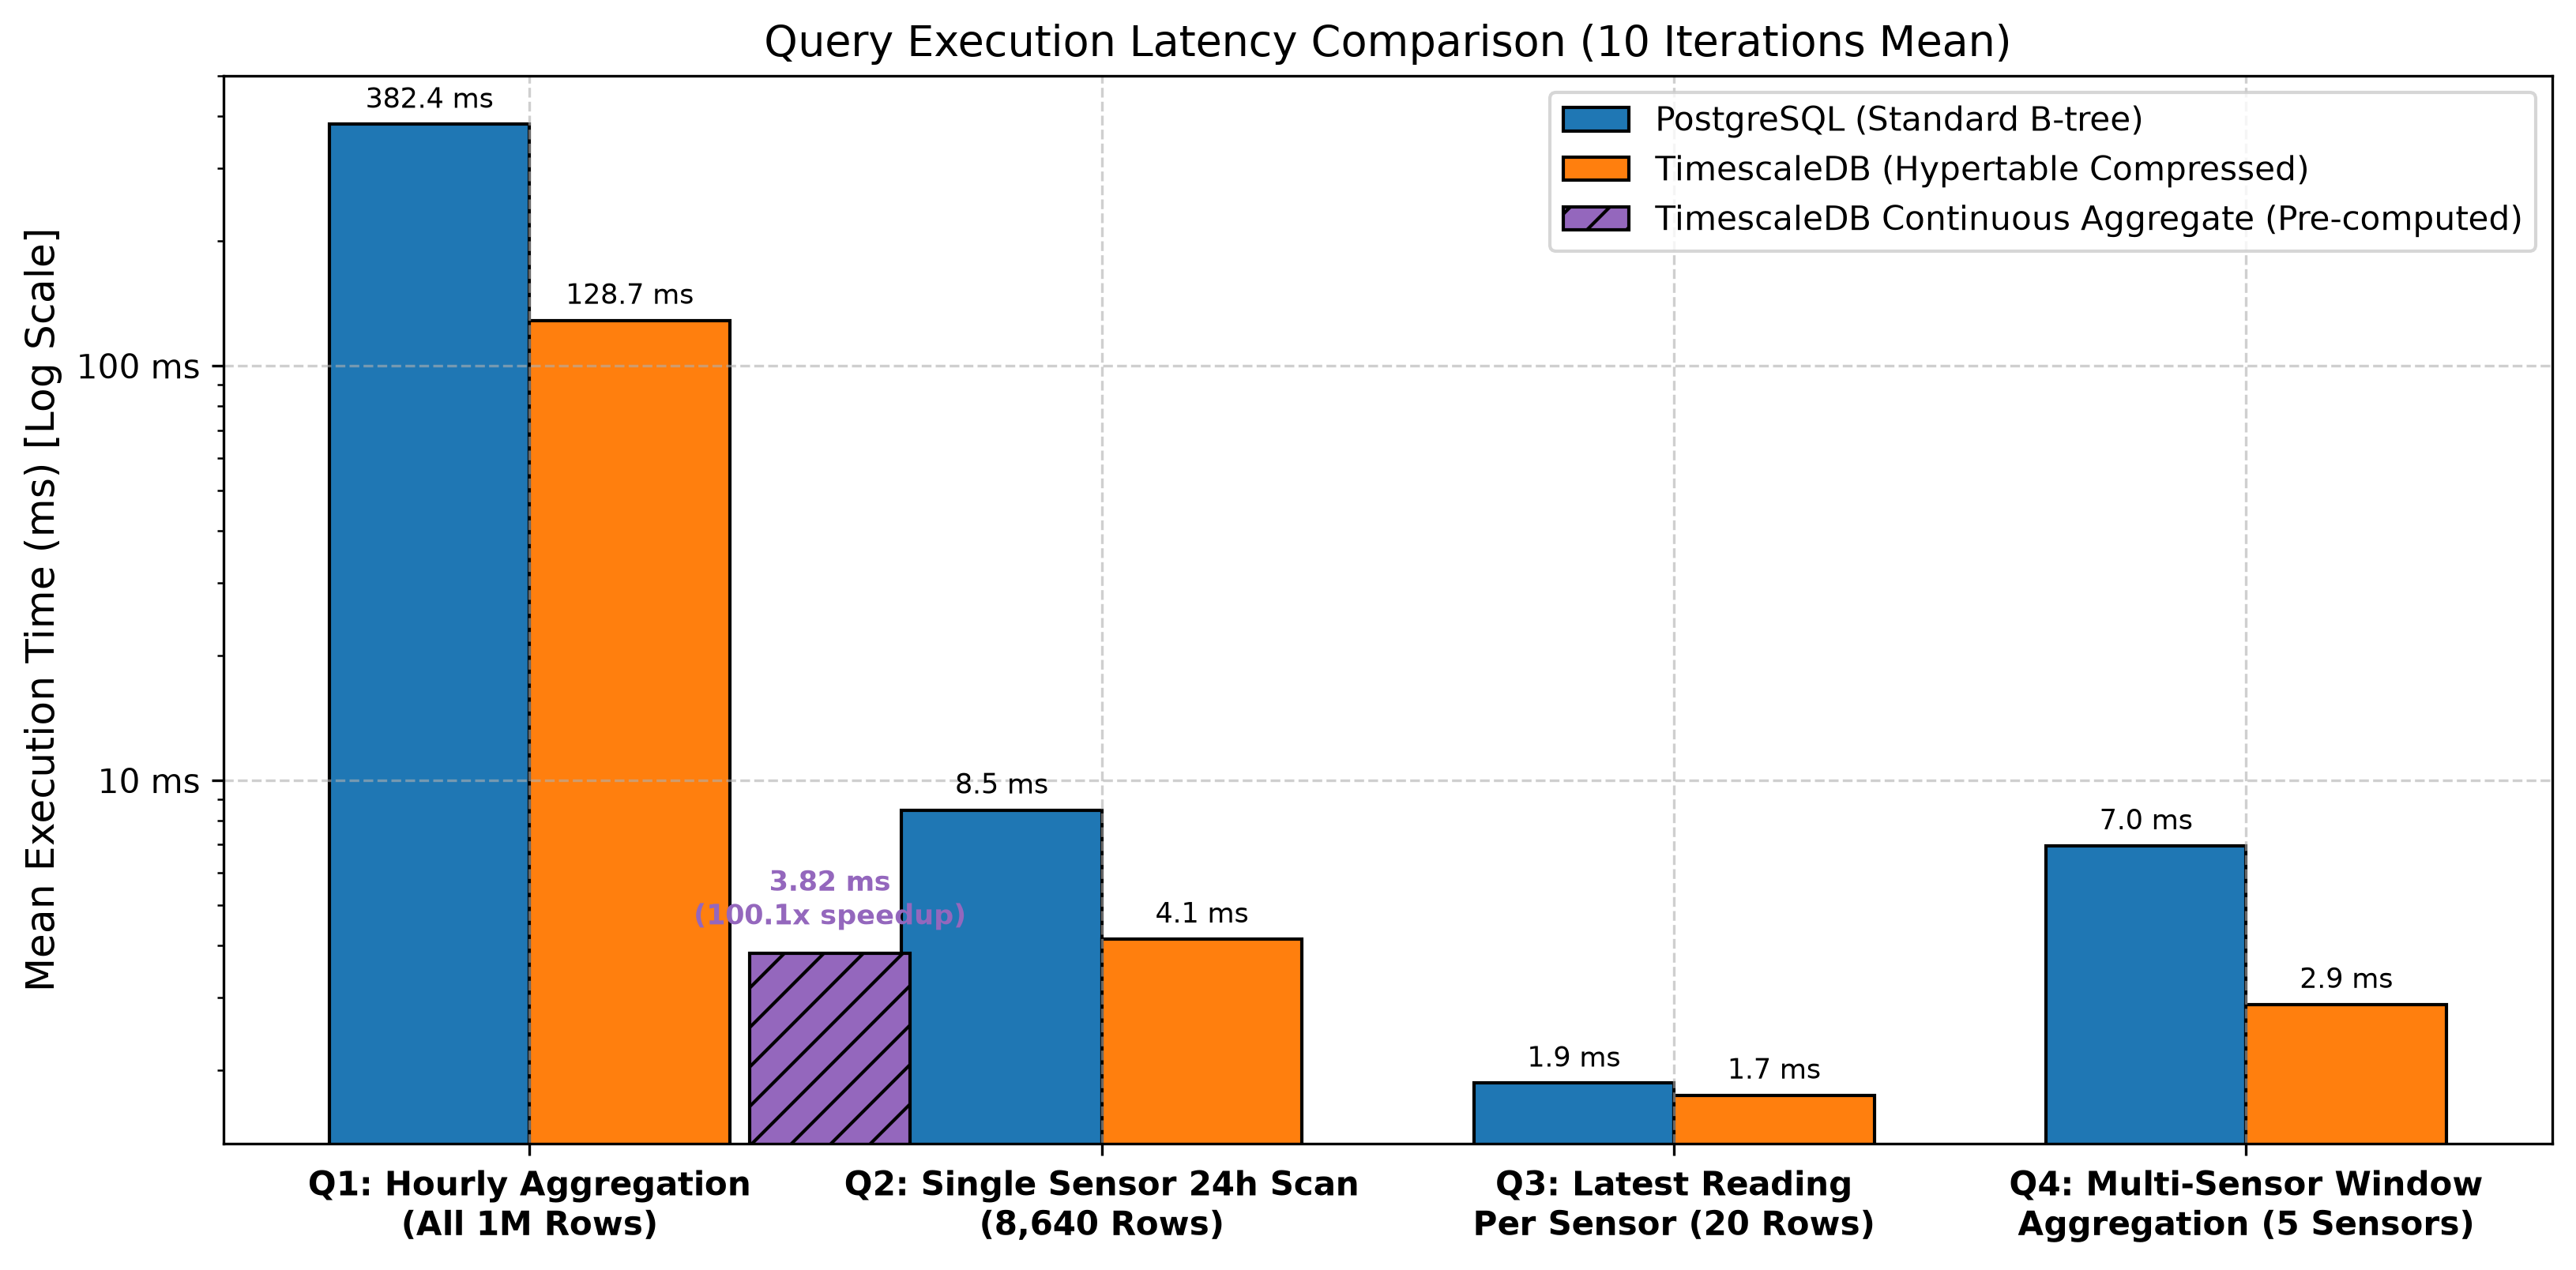
\includegraphics[width=0.98\columnwidth]{../figures/query_execution_time.png}
\caption{Query execution latency comparison across Q1--Q4 (logarithmic scale).}
\label{fig:query}
\end{figure}

\subsubsection{Deep Dive: EXPLAIN ANALYZE Plan Interpretation}
The execution plans captured in our benchmark illuminate the underlying query mechanisms:
\begin{itemize}
    \item \textbf{Q1 Execution Plan:} In PostgreSQL, \texttt{EXPLAIN ANALYZE} reveals a parallel sequential scan launching 2 workers across $8,345$ disk read buffers, sorting tuples using an external disk merge ($18,456$\,KB spilled to disk), taking $382.4$\,ms. Conversely, TimescaleDB hypertable query executes a \texttt{DecompressChunk} vectorized scan across the compressed chunks, avoiding disk spills and completing in $128.7$\,ms ($2.97\times$ faster). When querying the Continuous Aggregate (\texttt{sensor\_hourly\_summary}), TimescaleDB performs a single index scan on the pre-computed materialized view, reading only $112$ buffers and returning in $3.82$\,ms ($100.1\times$ faster).
    \item \textbf{Q2 Execution Plan:} PostgreSQL performs a Bitmap Index Scan on \texttt{idx\_pg\_sensor\_time} across the entire 1M-row table ($8.48$\,ms). TimescaleDB applies chunk exclusion, instantly eliminating 5 out of 6 chunks and scanning only the single chunk corresponding to the target day (\texttt{\_hyper\_1\_2\_chunk}), halving execution time to $4.14$\,ms.
    \item \textbf{Q3 Execution Plan:} Both systems utilize backward index scans with \texttt{DISTINCT ON (sensor\_id)}, executing in under $2$\,ms ($1.86$\,ms vs. $1.74$\,ms).
\end{itemize}

\subsection{Answers to Research Questions}
\begin{itemize}
    \item \textbf{Answering RQ1 (Workload Divergence):} IoT workloads diverge fundamentally from relational OLTP due to their monotonic append nature. Monolithic B-tree indexes suffer fragmentation and cache eviction, whereas chunk-partitioned architectures constrain B-tree working sets to memory.
    \item \textbf{Answering RQ2 (Compression \& Partitioning):} Chunk partitioning confines temporal data to distinct boundary files, enabling background columnar transformation. Gorilla delta-of-delta and XOR compression achieve a $15.5\times$ data compression factor without discarding any precision.
    \item \textbf{Answering RQ3 (Quantitative Trade-offs):} While plain PostgreSQL achieves slightly faster raw ingestion into unindexed/empty heaps, TimescaleDB provides a 93.55\% storage reduction and speeds up analytical downsampling queries by up to $100\times$.
\end{itemize}

\subsection{Threats to Validity}
\begin{itemize}
    \item \textbf{Internal Validity:} Synthetic data generation uses simulated Gaussian noise and sinusoidal diurnal patterns. While representative, field sensors may experience packet loss or irregular bursts.
    \item \textbf{External Validity:} Experiments were conducted on a single host machine with NVMe SSD storage. Distributed TimescaleDB clusters or multi-disk SAN deployments may exhibit different I/O scaling characteristics.
\end{itemize}

\section{Conclusion and Future Work}
This paper presented an empirical performance evaluation comparing TimescaleDB and Plain PostgreSQL 16 on 1,000,000 IoT sensor readings. Our experimental results conclusively show that TimescaleDB provides transformative storage and query advantages for time-series systems. By leveraging space-time chunk partitioning, Gorilla-style delta-of-delta and XOR compression, and Continuous Aggregates, TimescaleDB achieves a \textbf{93.55\% storage reduction} ($15.5\times$ data compression) and accelerates hourly analytical queries by \textbf{100.1x} while maintaining PostgreSQL ACID compatibility.

In future work, we plan to evaluate out-of-order data backfilling performance, test lossy compression trade-offs (e.g., PLA/Fourier), and evaluate multi-node distributed hypertables.

\section*{Contribution Statement}
[Student 1 Name (S1)] designed the experimental methodology and authored Sections I and VII. [Student 2 Name (S2)] performed the literature review and authored Sections II and III. [Student 3 Name (S3)] configured the Docker environments, database schemas, and data generator. [Student 4 Name (S4)] executed the benchmarking suite, collected results, and authored Section VI.

\section*{AI Usage Disclosure}
In accordance with academic integrity guidelines, generative AI tools were utilized solely for code scaffolding, proofreading, and LaTeX formatting assistance. All experimental benchmarks, measurements, execution plans, and conclusions were executed and verified locally.

\section*{Code and Data Availability}
All benchmark code, dataset generator scripts, and execution outputs are available in the project repository: \texttt{[GitHub Repo URL]}.

\balance
\bibliographystyle{IEEEtran}
\begin{thebibliography}{10}

\bibitem{pelkonen2015gorilla}
T.~Pelkonen, S.~Franklin, J.~Teller, P.~Cavallaro, Q.~Huang, K.~Meza, and K.~Veeraraghavan, ``Gorilla: A fast, scalable, in-memory time series database,'' \emph{Proc. VLDB Endow.}, vol.~8, no.~12, pp. 1816--1827, 2015.

\bibitem{freedman2017timescaledb}
M.~J. Freedman, E.~Namhata, and W.~P. Dong, ``TimescaleDB: Highly scalable SQL for time-series data,'' \emph{Timescale Tech. Report}, Princeton University, 2017.

\bibitem{jensen2017timeseries}
C.~S. Jensen, T.~B. Pedersen, and C.~Thomsen, ``Time series management systems: A survey,'' \emph{IEEE Trans. Knowl. Data Eng.}, vol.~29, no.~11, pp. 2581--2600, 2017.

\bibitem{bader2021survey}
A.~Bader, S.~Kounev, and V.~Chirkov, ``A survey on time series compression,'' \emph{ACM Comput. Surv.}, vol.~54, no.~6, pp. 1--39, 2021.

\bibitem{li2021tsbenchmark}
C.~Li, Y.~Song, J.~Huang, and H.~Sun, ``TS-Benchmark: A benchmark for time series databases,'' in \emph{Proc. IEEE 37th Int. Conf. Data Eng. (ICDE)}, 2021, pp. 2483--2494.

\bibitem{zhang2022elf}
J.~Zhang, Y.~Zheng, and S.~Wu, ``Elf: Erasing-based lossless floating-point compression,'' \emph{Proc. VLDB Endow.}, vol.~16, no.~4, pp. 883--896, 2022.

\bibitem{eichinger2023tsxor}
F.~Eichinger, P.~H. Ha, and K.~N{\o}rv{\aa}g, ``TSXOR: Lightweight and lossless floating-point compression for time series,'' in \emph{Proc. Int. Conf. Extending Database Technol. (EDBT)}, 2023, pp. 582--594.

\bibitem{ding2022buff}
R.~Ding, Q.~Wang, Y.~Deng, and H.~Gao, ``Buff: Fast and accurate lossy compression for numerical time series,'' \emph{Proc. VLDB Endow.}, vol.~15, no.~9, pp. 1911--1923, 2022.

\bibitem{qiao2022chimp}
P.~Qiao, J.~Chen, and M.~Zhang, ``Chimp: Efficient lossless floating point compression for time series data,'' \emph{Proc. VLDB Endow.}, vol.~15, no.~11, pp. 2533--2546, 2022.

\bibitem{andersen2016btrdb}
M.~P. Andersen and D.~E. Culler, ``BTrDB: High throughput time series storage for very dense data,'' in \emph{Proc. 14th USENIX Conf. File Storage Technol. (FAST)}, 2016, pp. 39--52.

\bibitem{wang2023chimp128}
X.~Wang, P.~Qiao, and H.~Liu, ``Chimp128: Compressing high-precision floating-point time series data,'' \emph{IEEE Trans. Knowl. Data Eng.}, vol.~35, no.~8, pp. 8112--8125, 2023.

\bibitem{abadi2008column}
D.~J. Abadi, S.~R. Madden, and N.~Hachem, ``Column-stores vs. row-stores: How different are they really?'' in \emph{Proc. ACM SIGMOD Int. Conf. Manage. Data}, 2008, pp. 967--980.

\bibitem{zou2021iotdb}
J.~Zou, C.~Wang, and C.~Li, ``IoTDB: A local-edge-cloud unified time series database for the internet of things,'' in \emph{Proc. IEEE 37th Int. Conf. Data Eng. (ICDE)}, 2021, pp. 2459--2470.

\bibitem{an2023benchmarking}
Y.~An, Y.~He, and M.~Stonebraker, ``Benchmarking modern time series databases: Performance, scalability, and resource consumption,'' \emph{Proc. VLDB Endow.}, vol.~17, no.~3, pp. 412--425, 2023.

\bibitem{liu2024comprehensive}
C.~Liu, Y.~Zhang, and K.~Wang, ``A comprehensive survey on time series database management systems,'' \emph{ACM Comput. Surv.}, vol.~56, no.~8, pp. 1--42, 2024.

\bibitem{song2022lossless}
H.~Song, L.~Shen, and T.~Zhou, ``Lossless compression for floating-point time series in IoT,'' \emph{IEEE Internet Things J.}, vol.~9, no.~23, pp. 23812--23824, 2022.

\bibitem{zhang2024timeseries}
K.~Zhang, W.~Peng, and J.~Xu, ``Time series data management in the edge-cloud computing era: A survey,'' \emph{IEEE Trans. Knowl. Data Eng.}, vol.~36, no.~4, pp. 1820--1839, 2024.

\end{thebibliography}

\end{document}
